\section{Location based Services in der Praxis}
	\subsection{Anwendungsbereiche}
Location Based Services, also mobile, positionsbezogene Dienste haben allgemein ein sehr breites Einsatzgebiet.\\
\paragraph{Theoretische Einsatzgebiete}
Der Autoren Allan J Brimicombe und Chao Li unterscheiden in ihrem Buch "'Location-Based Services and Geo-Information Engineering"' ~\cite[S.132]{brimicombe_li:application_area} zehn verschiedene Einsatzgebiete:
\begin{itemize}
	\item Navigation\\
Navigation ist die gezielte Führung des Nutzers von Punkt A nach Punkt B. Einige Geräte bieten auch eine Echtzeit-Analyse an.
	\item Wegfindung\\
Bei der Wegfindung hingegen liegt der Fokus auf dem Finden möglicher Wege, d.h. sie dient der allgemeinen Orientierung des Nutzers.
	\item Echtzeit-Verfolgung\\
Verfolgungs- auch Tracking-Systeme genannt, dienen der Echtzeitanalyse des Nutzerstandorts, um diesem z.B. das Finden von Freunden in der näheren Umgebung zu erleichtern.
	\item Elektronischer Handel\\
Bei Anwendungen aus dem Bereich des elektronischen Handel, auch E-Commerce genannt, handelt es sich um werbende Produkte, die dem Nutzer auf Basis seiner Position ortsspezifische Angebote eröffnen.
	\item User-solicited Informations (vom Nutzer gewünschte Informationen)\\
Unter diese Kategorie fallen alle Anwendungen, die vom Nutzer für den geschäftlichen oder sozialen Gebrauch genutzt werden. Beispiele dafür sind: Wetterprognosen, Zugverspätungen und Filmvorführungen.
	\item Ortsgebundene Tarife
	\item Fulfilment
	\item Koordination
	\item Kunstvoller Ausdruck
	\item Mobile Spiele
\end{itemize}

\paragraph{Praktische Einsatzgebiete}
Nach einer Goldmedia-Analyse~\cite[S.9]{goldmedia:lbs} verteilten sich die deutsche LBS-Marktstruktur 2014 auf 15 unterschiedliche Gebiete.\\
In der Studie werden folgende Punkte unterschieden:
\begin{itemize}
	\item Tourismus
	\item Beförderung und Verkehr
	\item Navigation und Maps
	\item Gastronomie
	\item Couponing und Einkauf
	\item Social
	\item Taxi
	\item Sport
	\item Augmented Reality
	\item Allgemeine Informationen
	\item Carsharing
	\item Gaming
	\item Gesundheit
	\item Media
	\item Sonstiges
\end{itemize}
Ganz offensichtlich ist diese Unterteilung vielschichtiger als die von Allan J Brimicombe und Chao Li. Es werden jeweils andere Schwerpunkte gesetzt. Es gibt jedoch auch Gemeinsamkeiten.

\paragraph{Gemeinsamkeiten und Unterschiede}
Navigation ist ein wichtiger Punkt in beiden Übersichten. Den Standort anzuzeigen bzw. den Nutzer zu navigieren ist eine der ersten Anwendungsbereiche von LBS.
	\subsection{Typen von Location based Services (proaktiv und reaktiv)}
Typen
	\subsubsection{Typen Teil 1}
...
	\subsection{Location based Services auf mobilen Endgeräten}
Beispie

\section{Kartenmaterial im Browser / Hybridapp}

Kartenmaterial im Browser bzw. der Hybrid-App ist ein essentieller Bestandteil von Location based Services. Durch eine Positionsbestimmung alleine erhält man nur Daten die für den Nutzer nicht anschaulich sind. Diese liegen normalerweise als geografische Koordinaten vor, die in geografischer Breite und geografischer Länge angegeben werden. Eine Beispielposition soll die Bedeutung von Kartenmaterial für den Nutzer von Location based Services verdeutlichen.

Als Beispiel hierfür wurde die Position der DHBW Mannheim in der Coblitzallee gewählt. Hierbei werden die geografischen Koordinaten, eine Adresse und ein Kartenausschnitt in einer Tabelle gegenübergestellt. Siehe hierzu Tabelle \ref{BedeutungVonKartenmaterial}.

\begin{table}[hb]
\begin{center}
\begin{tabular}{|p{4.75cm}p{4.75cm}p{4.75cm}|} 
	\hline
		\rowcolor{black} \textcolor{white} { \textbf{Geographische Koordinaten} } & \textcolor{white}{\textbf{Adresse}} & \textcolor{white}{\textbf{Kartenausschnitt}}\\ 
		\rowcolor[gray]{.75}  49$^\circ$28'27.6\grqq N 8$^\circ$32'03.9\grqq E & Duale Hochschule Baden-Württemberg Mannheim \newline 
Coblitzallee 1-9 \newline 
68163 Mannheim \newline (Neuostheim) & Kartenausschnitt\newline 
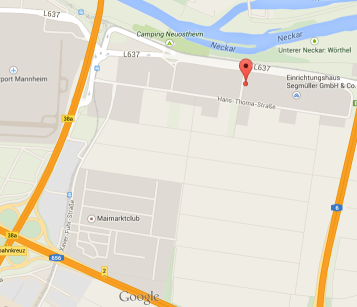
\includegraphics[width=0.3\textwidth]{ref/images/KartenmaterialKlein.png} \\ 
\hline
	\end{tabular}
\end{center}
\caption{Bedeutung von Kartenmaterial} \label{BedeutungVonKartenmaterial}
\end{table}

In der Tabelle sind verschiedenen Ortsdaten zur Verfügung gestellt, die alle Vor- und Nachteile aufweisen.

Die Geographischen Koordinaten geben die Position am genausten an, sind für fast keine Nutzer einer App von Bedeutung. 

Die Adresse ist im Alltag am geläufigsten und somit für Nutzer am verständlichsten. Allerdings ist die Angabe nicht so genau, wie die Geographischen Koordinaten. Denn die Angabe Hausnummer 1-9 gibt einen relativ großen Bereich an.

Die Vorteile eines Kartenausschnitts sind, dass die Detaillierung vom Nutzer angepasst werden kann. Des Weiteren werden viele grafische Informationen angezeigt, wie zum Beispiel der eigene Standort, an denen sich ein Nutzer Orientieren kann. Der Nachteil dieser Variante ist, dass die Kartenausschnitte die Zuhilfenahme von externen Quellen und einem erhöhten TODO: Programmieraufwand mit sich bringen.


TODO: Quelle finden
Auf Smartphones gehört Kartenmaterial und dessen Integration in Apps mittlerweile zum Standard, an welchen sich Nutzer gewöhnt haben. Aus diesem Grund sollte auch Kartenmaterial in die Location based Services App integriert werden, welche die Autoren bei dieser Studienarbeit entwickeln. 

Mögliche Quellen für das Kartenmaterial sind \glqq Google Maps\grqq, \glqq Bing Maps\grqq  und \glqq Open Street Maps\grqq.


\subsection{Google Maps}

\subsection{Bing Maps}

\subsection{Open Street Maps}







	\subsubsection{Aufzählen vieler Anwendungsbeispiele mit Erläuterung des Nutzens}
...
	\subsubsection{Umsetzungsmöglichkeiten für die Beispiele nennen}
...